% !TEX root = Master.tex


So far we explored the data addressing multiple characteristics of article unit sales along with other features in an aggregate or grouped frame. This section briefly highlights some additional aspects of demand quantities regarding individual articles and the associated limitations.
\\

Straight away, the biggest challenge is the life cycle of the articles, which is shown on the basis of seven exemplary articles. The course of those article sales is plotted in \autoref{fig:article_sample}. Article "5040" for example has only a lifespan of a 18 weeks and there are 12,679 out of 26,203 distinct articles having even less than that, which is almost half of the dataset. There are thousands of articles which have a lifespan of single digit (in weeks). The barplot in \autoref{fig:article_lifespan} makes the extent of this issue visible. Articles that were observed during the entire observation window (or at least the majority of it) are the exception to the rule. It should be mentioned also that many articles started their selling journey on eCom before 2017 where the data for this task were acquired and other articles are still being in stock after 2018. These troublesome facts make it very hard to apply any kind of promising quantitative methods. Nevertheless, this issue is discussed and tackled in later parts of this thesis (see Section \ref{ssec:article_dependencies}). It should be pointed out that for sales of many individual article, high peaks can be regularly observed during Black Friday periods too.
\\


\begin{figure}[H]
\centering
  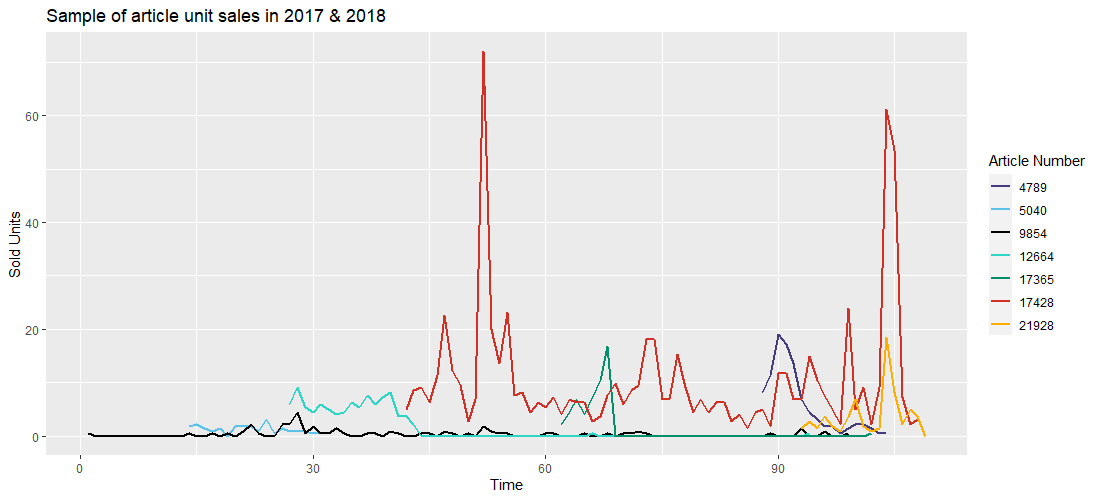
\includegraphics[width=0.95\linewidth]{figures/article_sample.png}
  \caption{Sample of seven articles and their demand quantity life cycles}
  \label{fig:article_sample}
\end{figure}


\begin{figure}[H]
\centering
  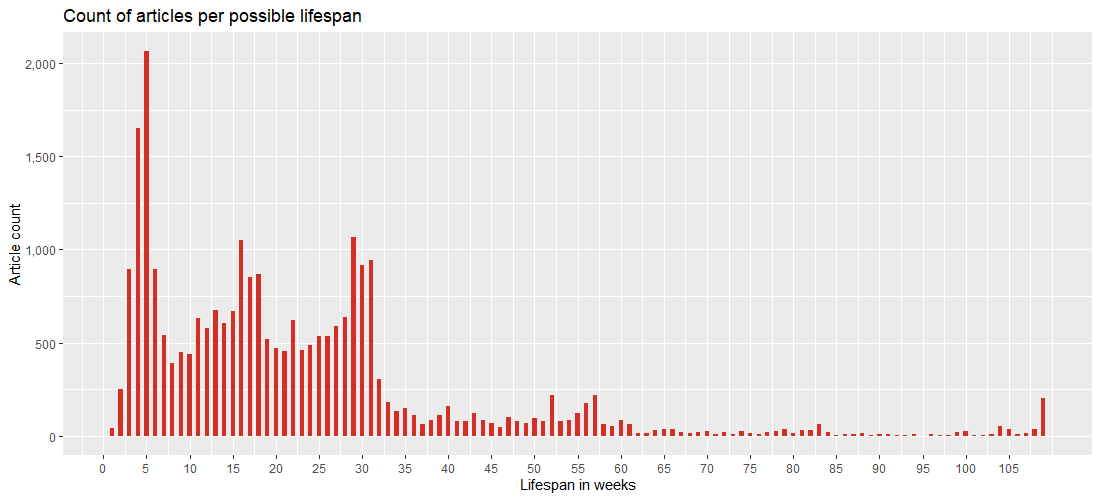
\includegraphics[width=0.95\linewidth]{figures/article_lifespan.png}
  \caption{Number of articles for each possible lifespan of 1 to 109 weeks}
  \label{fig:article_lifespan}
\end{figure}



Yet another immediate remark is the zero inflation persisting in the data. A lot of articles spend their time on eCom for several weeks without being sold once, as can be seen e.g. in \autoref{fig:article_sample} for articles "9854", "12664" and "17365". To be precise, for 100,732 instances we have a gross demand quantity of zero, which makes up almost a fifth of the dataset. Combining this inflation of zeros with the short lifespan increases the level difficulty even more.






